\documentclass{article}

\usepackage{amsmath,amssymb}
\usepackage{tikz}
\usepackage{pgfplots}
\usepackage{xcolor}
\usepackage[left=2.1cm,right=3.1cm,bottom=3cm,footskip=0.75cm,headsep=0.5cm]{geometry}
\usepackage{enumerate}
\usepackage{enumitem}
\usepackage{marvosym}
\usepackage{tabularx}
\usepackage{multirow}
\usepackage[colorlinks = true, linkcolor = blue, urlcolor  = blue, citecolor = blue, anchorcolor = blue]{hyperref}

\usepackage{listings}
\definecolor{lightlightgray}{rgb}{0.95,0.95,0.95}
\definecolor{lila}{rgb}{0.8,0,0.8}
\definecolor{mygray}{rgb}{0.5,0.5,0.5}
\definecolor{mygreen}{rgb}{0,0.8,0.26}
\lstdefinestyle{java} {language=java}
\lstset{language=java,
	basicstyle=\ttfamily,
	keywordstyle=\color{lila},
	commentstyle=\color{lightgray},
	stringstyle=\color{mygreen}\ttfamily,
	backgroundcolor=\color{white},
	showstringspaces=false,
	numbers=left,
	numbersep=10pt,
	numberstyle=\color{mygray}\ttfamily,
	identifierstyle=\color{blue},
	xleftmargin=.1\textwidth, 
	%xrightmargin=.1\textwidth,
	escapechar=§,
}

\usepackage[utf8]{inputenc}

\renewcommand*{\arraystretch}{1.4}

\newcolumntype{L}[1]{>{\raggedright\arraybackslash}p{#1}}
\newcolumntype{R}[1]{>{\raggedleft\arraybackslash}p{#1}}
\newcolumntype{C}[1]{>{\centering\let\newline\\\arraybackslash\hspace{0pt}}m{#1}}

\newcommand{\E}{\mathbb{E}}
\DeclareMathOperator{\rk}{rk}
\DeclareMathOperator{\Var}{Var}
\DeclareMathOperator{\Cov}{Cov}
\DeclareMathOperator{\SD}{SD}
\DeclareMathOperator{\Cor}{Cor}

\title{\textbf{Instrumente des Finanzmanagements, Übung 1}}
\author{\textsc{Henry Haustein}}
\date{}

\begin{document}
	\maketitle

	\section*{Aufgabe 10.4: Historische Erträge von Aktien und Anleihen}
	\begin{enumerate}[label=(\alph*)]
		\item Die Renditen sind
		\begin{itemize}
			\item bis 05.02.03: $r_1=\frac{30.67\text{ \EUR} - 33.88\text{ \EUR}}{33.88\text{ \EUR}} + \frac{0.17\text{ \EUR}}{33.88\text{ \EUR}} = -0.0897$
			\item bis 14.05.03: $r_2=\frac{29.49\text{ \EUR} - 30.67\text{ \EUR}}{30.67\text{ \EUR}} + \frac{0.17\text{ \EUR}}{30.67\text{ \EUR}} = -0.0329$
			\item bis 13.08.03: $r_3=\frac{32.88\text{ \EUR} - 29.49\text{ \EUR}}{29.49\text{ \EUR}} + \frac{0.17\text{ \EUR}}{29.49\text{ \EUR}} = 0.1038$
			\item bis 12.11.03: $r_4=\frac{39.07\text{ \EUR} - 32.38\text{ \EUR}}{32.38\text{ \EUR}} + \frac{0.17\text{ \EUR}}{32.38\text{ \EUR}} = 0.2119$
			\item bis 02.01.04: $r_5=\frac{61.99\text{ \EUR} - 39.07\text{ \EUR}}{39.07\text{ \EUR}} = 0.0747$
		\end{itemize}
		Die Gesamtrendite ist dann
		\begin{align}
			r &= \prod_{i=1}^{5} (1+r_i) - 1 \notag \\
			&= (1-0.0897)(1-0.0329)(1+0.1038)(1+0.2119)(1+0.0747) - 1 \notag \\
			&= 0.2656 \notag
		\end{align}
		\item Die Renditen sind
		\begin{itemize}
			\item bis 06.02.08: $r_1=\frac{79.91\text{ \EUR} - 86.62\text{ \EUR}}{86.62\text{ \EUR}} + \frac{0.40\text{ \EUR}}{86.62\text{ \EUR}} = -0.0728$
			\item bis 07.05.08: $r_2=\frac{84.55\text{ \EUR} - 79.91\text{ \EUR}}{79.91\text{ \EUR}} + \frac{0.40\text{ \EUR}}{79.91\text{ \EUR}} = 0.0631$
			\item bis 06.08.08: $r_3=\frac{65.40\text{ \EUR} - 84.55\text{ \EUR}}{84.55\text{ \EUR}} + \frac{0.40\text{ \EUR}}{84.55\text{ \EUR}} = -0.2218$
			\item bis 05.11.08: $r_4=\frac{49.55\text{ \EUR} - 65.40\text{ \EUR}}{65.40\text{ \EUR}} + \frac{0.40\text{ \EUR}}{65.40\text{ \EUR}} = -0.2362$
			\item bis 02.01.09: $r_5=\frac{45.25\text{ \EUR} - 49.55\text{ \EUR}}{49.55\text{ \EUR}} = -0.0868$
		\end{itemize}
		Die Gesamtrendite ist dann
		\begin{align}
			r &= \prod_{i=1}^{5} (1+r_i) - 1 \notag \\
			&= (1-0.0728)(1+0.0631)(1-0.2218)(1-0.2362)(1-0.0868) - 1 \notag \\
			&= -0.4650 \notag
		\end{align}
	\end{enumerate}
	
	\section*{Aufgabe 10.5: Historische Erträge von Aktien und Anleihen}
	\begin{enumerate}[label=(\alph*)]
		\item $r=\sqrt[4]{1.1\cdot 1.2\cdot 0.95\cdot 1.15}-1=0.0958$
		\item $r=\frac{1.1+1.2+0.95+1.15}{4}=0.1$
		\item Performance in der Vergangenheit: geometrisch, Renditen unabhängig und gleichwahrscheinlich: arithmetisch
	\end{enumerate}
	
	\section*{Aufgabe 10.12: Diversifikation von Aktienportfolios}
	\begin{enumerate}[label=(\alph*)]
		\item Der Markt hat eine erwartete Rendite von 10 \%. Investiert man nach Methode (i), so kann man nach 2 Jahren $\E(r_{(i)}) = 1.05\cdot 1.1= 1.155 \Rightarrow 15.5$ \% erwarten. Für Methode (ii) gilt $\E(r_{(ii)}) = 1.1\cdot 1.1= 1.21 \Rightarrow 21$ \%.
		\item Folgt man Strategie (i), so kann der Markt im 2. Jahr entweder fallen oder steigen:
		\begin{center}
			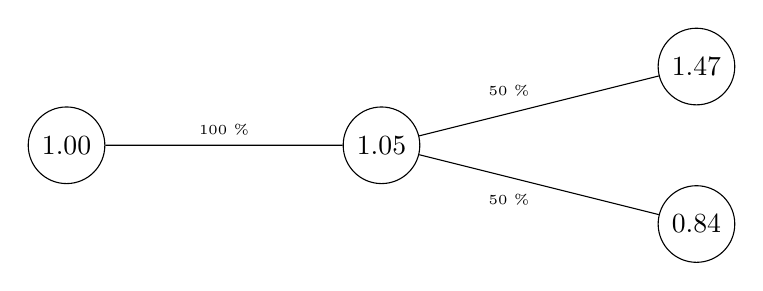
\begin{tikzpicture}
				\node[circle,draw=black, fill=white] (1) at (0,0) {1.00};
				\node[circle,draw=black, fill=white] (105) at (4,0) {1.05};
				\node[circle,draw=black, fill=white] (084) at (8,-1) {0.84};
				\node[circle,draw=black, fill=white] (147) at (8,1) {1.47};
				
				\draw (1) to node[above] {\tiny 100 \%} (105) to node[above left] {\tiny 50 \%} (147);
				\draw (105) to node[below left] {\tiny 50 \%} (084);
			\end{tikzpicture}
		\end{center}
		Die Standardabweichung ist damit 
		\begin{align}
			\SD(r_{(i)}) = \sqrt{0.5(1.47-1.155)^2 + 0.5(0.84-1.155)^2} = 0.315 \notag
		\end{align}
		Bei der Strategie (ii) kann der Markt in beiden Jahren steigen oder fallen:
		\begin{center}
			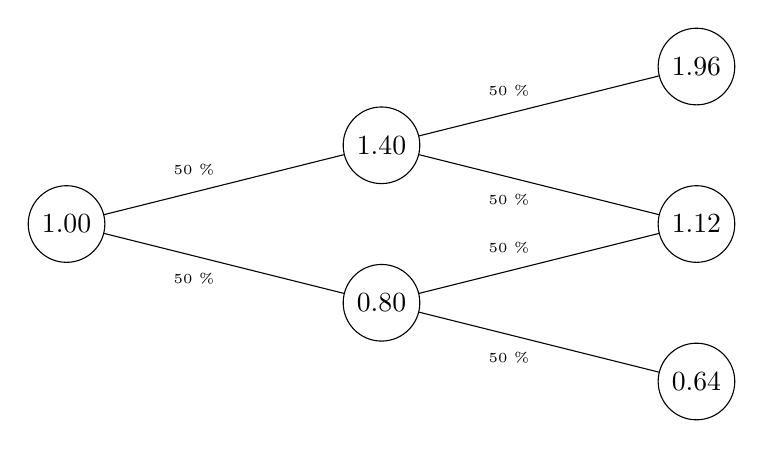
\begin{tikzpicture}
				\node[circle,draw=black, fill=white] (100) at (0,0) {1.00};
				\node[circle,draw=black, fill=white] (080) at (4,-1) {0.80};
				\node[circle,draw=black, fill=white] (140) at (4,1) {1.40};
				\node[circle,draw=black, fill=white] (064) at (8,-2) {0.64};
				\node[circle,draw=black, fill=white] (112) at (8,0) {1.12};
				\node[circle,draw=black, fill=white] (196) at (8,2) {1.96};
				
				\draw (100) to node[above left] {\tiny 50 \%} (140) to node[above left] {\tiny 50 \%} (196);
				\draw (100) to node[below left] {\tiny 50 \%} (080) to node[below left] {\tiny 50 \%} (064);
				\draw (140) to node[below left] {\tiny 50 \%} (112);
				\draw (080) to node[above left] {\tiny 50 \%} (112);
			\end{tikzpicture}
		\end{center}
		Die Standardabweichung ist damit 
		\begin{align}
			\SD(r_{(ii)}) = \sqrt{0.25(1.96-1.21)^2 + 0.5(1.12-1.21)^2 + 0.25(0.64-1.21)^2} = 0.4753 \notag
		\end{align}
		\item nein, es steigt
	\end{enumerate}

	\section*{Aufgabe 11.3: Die erwartete Rendite eines Portfolios}
	\begin{enumerate}[label=(\alph*)]
		\item $100\text{ Mio. Aktien}\cdot 100\text{ \EUR} + 50\text{ Mio. Aktien}\cdot 120\text{ \EUR} + 200\text{ Mio. Aktien} \cdot 3\text{ \EUR} = 22\text{ Mrd. \EUR}$
		\item Die Anteile sind
		\begin{align}
			\text{Anteil First Bank} &= \frac{100\text{ Mio. Aktien}\cdot 100\text{ \EUR}}{22\text{ Mrd. \EUR}} = 0.4545 \notag \\
			\text{Anteil Fast Mover} &= \frac{50\text{ Mio. Aktien}\cdot 120\text{ \EUR}}{22\text{ Mrd. \EUR}} = 0.2727 \notag \\
			\text{Anteil Funny Bone} &= \frac{200\text{ Mio. Aktien}\cdot 3\text{ \EUR}}{22\text{ Mrd. \EUR}} = 0.2727 \notag
		\end{align}
		\item $r=0.4545\cdot 0.18 + 0.2727\cdot 0.12 + 0.2727\cdot 0.15=0.1554$
	\end{enumerate}

	\section*{Aufgabe 11.8: Die Volatilität eines Portfolios aus zwei Aktien}
	\begin{enumerate}[label=(\alph*)]
		\item Wir müssen folgende Gleichung lösen. $\alpha$ beschreibt den Anteil von Tex-Aktien im Portfolio:
		\begin{align}
			\Var(\text{Mex-Aktien}) &= \Var(\alpha\cdot\Var(\text{Tex-Aktien}) + (1-\alpha)\cdot\Var(\text{Mex-Aktien})) \notag \\
			0.2^2 &= \alpha^2\cdot 0.4^2 + (1-\alpha)^2\cdot 0.2^2 \notag \\
			\Rightarrow \alpha_1 &= 0 \notag \\
			\Rightarrow \alpha_2 &= 0.4 \notag
		\end{align}
		\item Für das Minimum-Varianz-Portfolio (bei unkorrelierten Aktien) sind die Anteile
		\begin{align}
			\text{Anteil Tex} &= \frac{\Var(\text{Mex-Aktien})}{\Var(\text{Mex-Aktien}) + \Var(\text{Tex-Aktien})} = \frac{0.2^2}{0.4^2 + 0.2^2} = 0.2 \notag \\
			\text{Anteil Mex} &= \frac{\Var(\text{Tex-Aktien})}{\Var(\text{Mex-Aktien}) + \Var(\text{Tex-Aktien})} = \frac{0.4^2}{0.4^2 + 0.2^2} = 0.8 \notag
		\end{align}
	\end{enumerate}

	\section*{Aufgabe 416.2: Erwartete Rendite und SA eines Portfolios}
	\begin{enumerate}[label=(\alph*)]
		\item Die Anteile der einzelnen Aktien sind:
		\begin{align}
			\text{Anteil Oracle} &= \frac{-35\text{ Mio. \EUR}}{85\text{ Mio. \EUR} - 35\text{ Mio. \EUR}} = -0.7 \notag \\
			\text{Anteil Intel} &= \frac{85\text{ Mio. \EUR}}{85\text{ Mio. \EUR} - 35\text{ Mio. \EUR}} = 1.7 \notag
		\end{align}
		Die Rendite ist damit
		\begin{align}
			r = -0.7\cdot 0.12 + 1.7\cdot 0.145 = 0.1625 \notag
		\end{align}
		\item Die Covarianz zwischen den beiden Aktien ist
		\begin{align}
			\Cov(r_O, r_I) = \Cor(r_O,r_I)\cdot \SD(r_O)\cdot\SD(r_I) = 0.117 \notag
		\end{align}
		Damit ist die Varianz des Portfolios $P$
		\begin{align}
			\Var(P) &= -0.7^2\cdot 0.45^2 + 1.7^2\cdot 0.4^2 + 2\cdot -0.7\cdot 1.7\cdot 0.117 \notag \\
			&= 0.2832 \notag \\
			\SD(P) &= \sqrt{0.2832} \notag \\
			&= 0.5321 \notag
		\end{align}
	\end{enumerate}
	
\end{document}